\documentclass[12pt,a4paper]{article}
\usepackage[utf8]{inputenc}
\usepackage[brazil]{babel}
\usepackage{graphicx}
\usepackage{amssymb, amsfonts, amsmath}
\usepackage{float}
\usepackage{enumerate}
\usepackage[top=2.5cm, bottom=2.5cm, left=1.25cm, right=1.25cm]{geometry}

\begin{document}
\pagestyle{empty}

\begin{center}
  \begin{tabular}{ccc}
    \begin{tabular}{c}
      
\includegraphics[scale=0.25]{../../biblioteca/imagem/brasao-de-armas-brasil} \\
    \end{tabular} & 
    \begin{tabular}{c}
      Ministério da Educação \\
      Universidade Federal dos Vales do Jequitinhonha e Mucuri \\
      Faculdade de Ciências Sociais, Aplicadas e Exatas - FACSAE \\
      Departamento de Ciências Exatas - DCEX \\
      Disciplina: Geometria Analítica \quad Semestre: 2020/1\\
      Prof. Me. Luiz C. M. de Aquino\\
    \end{tabular} &
    \begin{tabular}{c}
      
\includegraphics[scale=0.25]{../../biblioteca/imagem/logo-ufvjm} \\
    \end{tabular}
  \end{tabular}
\end{center}

\begin{center}
  \textbf{Lista I}
\end{center}

\begin{enumerate}

  \item Represente geometricamente dois vetores $\vec{u}$ e $\vec{v}$ que possuem
    \underline{\textbf{apenas}}:
  
    \begin{enumerate}[(a)]
      \item a mesma direção;
      \item o mesmo sentido e mesma direção;
      \item a mesma magnitude (ou comprimento) e mesma direção;
    \end{enumerate}
  
  \item Efetue as operações $\dfrac{1}{2}\vec{a} + 2\vec{b}$ e $-2\vec{c} + \vec{d}$
  com os vetores indicados abaixo, fazendo o esboço da representação gráfica do resultado.

  \begin{figure}[!htb]
    \centering
    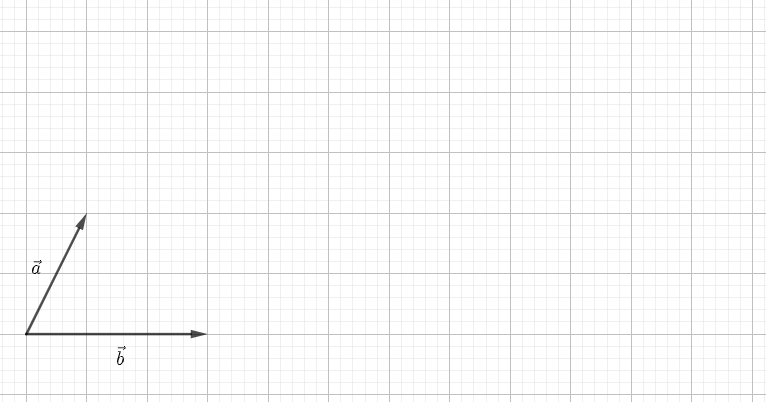
\includegraphics[scale=0.5]{imagem/lista-i-questao-1-a}
  \end{figure}

  \begin{figure}[!htb]
    \centering
    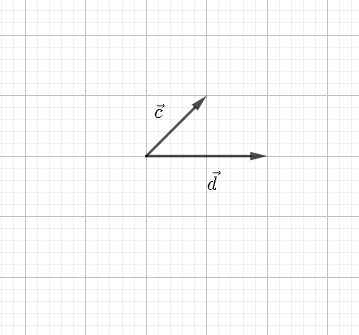
\includegraphics[scale=0.5]{imagem/lista-i-questao-1-b}
  \end{figure}

  \item A figura abaixo ilustra o cubo $ABCDEFGH$. Determine o resultado da operação:
    $\overrightarrow{BA} + \overrightarrow{HE} + \overrightarrow{CG}$.

  \begin{figure}[!htb]
    \centering
    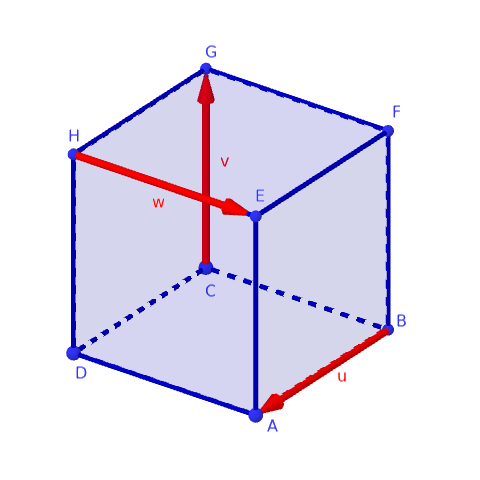
\includegraphics[scale=0.5]{imagem/cubo}
  \end{figure}
 
  \item Sejam quaisquer pontos $A$, $B$, $C$, $D$ e $E$. Determine o resultado da operação:
    $\overrightarrow{BA} - \overrightarrow{BD} + \overrightarrow{CD} - \overrightarrow{EA}$.
    Represente graficamente o seu resultado.
    
  \item Classifique as afirmações em Verdadeiro ou Falso.
  
  \begin{description}
    \item[(\quad)] O vetor $-2\vec{u}$ tem a mesma direção de $\vec{u}$, mas tem 
      sentido contrário.
    \item[(\quad)] O vetor $-2\vec{u}$ tem a metade do comprimento de $\vec{u}$.
    \item[(\quad)] Se $\vec{u}$ e $\vec{v}$ possuem a mesma direção, sentido e
      comprimento, então $\vec{u} = \vec{v}$.
    \item[(\quad)] Para qualquer vetor $\vec{u}$, temos que
      $\vec{u} + (-\vec{u}) = \vec{0}$.
    \item[(\quad)] Os vetores $\lambda u$ e $-\lambda u$ possuem comprimentos
      diferentes.
    \item[(\quad)] Sendo $A$, $B$, $C$ e $D$ pontos quaisquer, temos que 
      $\overrightarrow{AB} - \overrightarrow{CB} + \overrightarrow{CD} = \overrightarrow{AD}$.
  \end{description}

  \item Sejam $\overline{AB}$ e $\overline{CD}$ dois segmentos paralelos e de
  comprimento não nulo. Prove que $\overrightarrow{AB} = \lambda\overrightarrow{CD}$.
    
  \item Seja $ABC$ um triângulo com $M$ e $N$ os pontos médios de $\overline{AB}$ e
    $\overline{AC}$, respectivamente. Prove que $\overline{MN}$ é paralelo à
    $\overline{BC}$ e $\overline{MN} = \dfrac{1}{2}\overline{BC}$.
 
  \item Prove que as diagonais de um paralelogramo se cruzam ao meio. (Sugestão:
    considerando que $M$ e $N$ são os pontos médios das diagonais do paralelogramo, 
    prove que $\overrightarrow{MN} = \vec{0}$ e conclua que $M = N$.)
  
\end{enumerate}

\end{document}
